\documentclass[aspectratio=169,10pt]{beamer}

\usepackage[T1]{fontenc}
\usepackage{lmodern}
\usepackage{booktabs}
\usepackage{tabularx}
\usepackage{array}
\usepackage{tikz}
\usetikzlibrary{arrows.meta,positioning,fit}

\definecolor{HopkinsBlue}{HTML}{002D72}
\definecolor{SpiritBlue}{HTML}{68ACE5}
\definecolor{DeepBlue}{HTML}{001B44}
\definecolor{PaleBlue}{HTML}{EAF4FB}
\definecolor{Muted}{HTML}{526777}
\definecolor{Success}{HTML}{287A57}
\definecolor{Attention}{HTML}{B65738}
\definecolor{LightGray}{HTML}{EEF1F3}

\setbeamercolor{normal text}{fg=DeepBlue,bg=white}
\setbeamercolor{structure}{fg=HopkinsBlue}
\setbeamercolor{frametitle}{fg=white,bg=HopkinsBlue}
\setbeamercolor{title}{fg=HopkinsBlue}
\setbeamercolor{subtitle}{fg=Muted}
\setbeamercolor{block title}{fg=white,bg=HopkinsBlue}
\setbeamercolor{block body}{fg=DeepBlue,bg=PaleBlue}
\setbeamercolor{alerted text}{fg=Attention}
\setbeamertemplate{navigation symbols}{}
\setbeamertemplate{itemize item}{\color{SpiritBlue}$\blacktriangleright$}
\setbeamertemplate{itemize subitem}{\color{HopkinsBlue}$\bullet$}
\setbeamertemplate{enumerate item}{\color{HopkinsBlue}\insertenumlabel.}
\setbeamertemplate{footline}{%
  \leavevmode\hbox{%
    \begin{beamercolorbox}[wd=.82\paperwidth,ht=2.6ex,dp=1.1ex,leftskip=1em]{author in head/foot}%
      \color{Muted}\scriptsize Digital Professor --- Interaction and Evidence Module
    \end{beamercolorbox}%
    \begin{beamercolorbox}[wd=.18\paperwidth,ht=2.6ex,dp=1.1ex,rightskip=1em plus1fil]{date in head/foot}%
      \color{Muted}\scriptsize\hfill\insertframenumber/\inserttotalframenumber
    \end{beamercolorbox}}}
\setbeamertemplate{frametitle}{%
  \nointerlineskip
  \begin{beamercolorbox}[wd=\paperwidth,ht=3.15ex,dp=1.15ex,leftskip=.55cm]{frametitle}%
    \insertframetitle
  \end{beamercolorbox}}

\newcolumntype{Y}{>{\raggedright\arraybackslash}X}
\newcolumntype{P}[1]{>{\raggedright\arraybackslash}p{#1}}
\newcommand{\specnote}[2]{%
  \vfill\hfill{\tiny\color{Muted}Spec: \href{run:../../specs/#1}{\texttt{#1} #2}}}

\title{Interaction and Evidence Module}
\subtitle{A specification for capturing student work and coordinating a tutoring turn}
\author{Jonathan Ma}
\institute{Digital Professor}
\date{October 2026}

\begin{document}

% 0:20
\begin{frame}[plain]
  \vfill
  {\usebeamerfont{title}\color{HopkinsBlue}\LARGE\inserttitle\par}
  \vspace{.55em}
  {\color{Muted}\large\insertsubtitle\par}
  \vspace{1.4em}
  {\color{SpiritBlue}\rule{2.4cm}{2pt}}\par
  \vspace{1.2em}
  {\small\insertauthor\hfill\insertdate}
  \vfill
\end{frame}

% 1:10
\begin{frame}{Interaction's role in the system}
\small
\textbf{Goal:} capture student work without changing its meaning, confirm consequential ambiguity, and pass factual evidence through the tutoring loop.
\vspace{.45em}
\centering
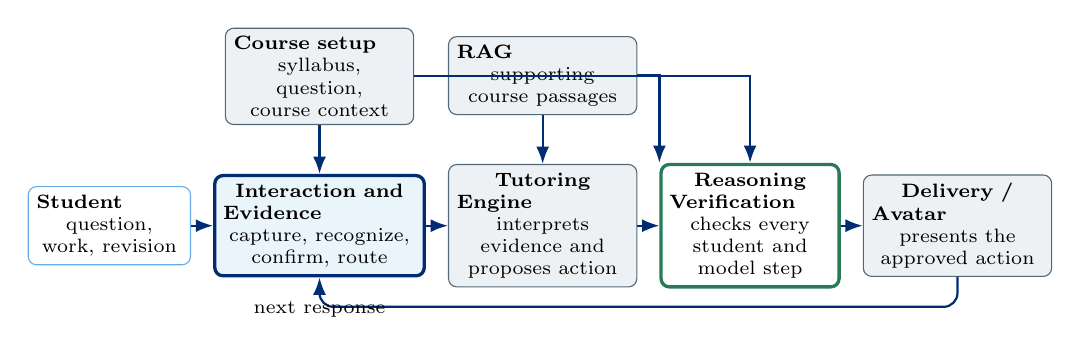
\begin{tikzpicture}[
  node distance=.42cm and .28cm,
  mine/.style={draw=HopkinsBlue,very thick,rounded corners=3pt,fill=PaleBlue,align=center,text width=2.45cm,minimum height=1.02cm,inner sep=3pt,font=\scriptsize},
  other/.style={draw=Muted,rounded corners=3pt,fill=LightGray,align=center,text width=2.18cm,minimum height=.90cm,inner sep=3pt,font=\scriptsize},
  check/.style={draw=Success,very thick,rounded corners=3pt,fill=white,align=center,text width=2.05cm,minimum height=.90cm,inner sep=3pt,font=\scriptsize},
  input/.style={draw=SpiritBlue,rounded corners=3pt,fill=white,align=center,text width=1.85cm,minimum height=.90cm,inner sep=3pt,font=\scriptsize},
  arrow/.style={-{Latex[length=2.2mm]},thick,draw=HopkinsBlue}]
\node[input] (student) {\textbf{Student}\newline question, work, revision};
\node[mine,right=of student] (interaction) {\textbf{Interaction and Evidence}\newline capture, recognize, confirm, route};
\node[other,right=of interaction] (engine) {\textbf{Tutoring Engine}\newline interprets evidence and proposes action};
\node[check,right=of engine] (verifier) {\textbf{Reasoning Verification}\newline checks every student and model step};
\node[other,right=of verifier] (delivery) {\textbf{Delivery / Avatar}\newline presents the approved action};
\node[other,above=.62cm of interaction] (context) {\textbf{Course setup}\newline syllabus, question, course context};
\node[other,above=.62cm of engine] (retrieval) {\textbf{RAG}\newline supporting course passages};
\draw[arrow] (student)--(interaction);
\draw[arrow] (interaction)--(engine);
\draw[arrow] (engine)--(verifier);
\draw[arrow] (verifier)--(delivery);
\draw[arrow] (context)--(interaction);
\draw[arrow] (retrieval)--(engine);
\draw[arrow] (context.east) -| (verifier.north);
\draw[arrow] (retrieval.east) -| (verifier.north west);
\draw[arrow,rounded corners=5pt] (delivery.south) -- ++(0,-.38) -| node[pos=.76,below,font=\scriptsize]{next response} (interaction.south);
\end{tikzpicture}
\vspace{.35em}

\textbf{Interaction owns the blue box only.} It does not ingest course content, retrieve passages, diagnose learning, choose or verify tutoring actions, or control avatar presentation.
\specnote{architecture.md}{\S\S3--5; \texttt{student-interaction.md} \S\S1--2}
\end{frame}

% 1:10
\begin{frame}{V1 scope and ownership boundary}
\small
\begin{columns}[T,onlytextwidth]
\column{.48\textwidth}
\begin{block}{V1 student inputs}
\begin{itemize}
\item Typed text, Markdown, code, and TeX
\item Handwritten image/PDF with a preserved original and logged resolution/contrast enhancement
\item Direct stylus input through a sketchpad
\item One recorded voice clip with editable transcript
\end{itemize}
\end{block}
\begin{block}{Deferred}
Continuous voice, live video, and real-time avatar conversation.
\end{block}
\column{.49\textwidth}
\begin{block}{Interaction owns}
Capture, recognition routing, focused confirmation, Student Evidence construction, attempt links, and handoff status.
\end{block}
\begin{block}{Other modules own}
Course ingestion, RAG ranking, learner diagnosis, tutoring-action selection, reasoning verification, and presentation.
\end{block}
\end{columns}
\vspace{.35em}
\centering
\textbf{Design rule:} coordinate the turn without duplicating another module's decision.
\specnote{student-interaction.md}{\S\S2--4; \texttt{architecture.md} \S4}
\end{frame}

% 1:20
\begin{frame}{Inputs: what arrives and from where}
\footnotesize
\begin{tabularx}{\textwidth}{@{}P{.25\textwidth}P{.26\textwidth}Y@{}}
\toprule
\textbf{Input} & \textbf{Producing module} & \textbf{Interaction uses} \\
\midrule
Student submission & Student/client & Original work, input type, explanation, and stated uncertainty. \\
\addlinespace
Course/question references & Course Context/Ingestion & IDs, display-safe prompt, allowed response modes, and constraints. \\
\addlinespace
Recognition response & Interaction recognizer & Transcription, alternatives, ambiguous regions, model version, and status. \\
\addlinespace
Tutoring Action + verification & Tutoring Engine + Reasoning Verification & Approved action, per-step verification status, and expected response; forwarded unchanged. \\
\addlinespace
Delivery Result & Delivery Layer/Avatar & Presented content, channel, available response modes, and delivery status. \\
\addlinespace
Logging configuration & System/session configuration & Logging, retention, redaction, and cost settings. \\
\bottomrule
\end{tabularx}
\vspace{.35em}
\centering
\textbf{Restricted:} expected solutions and diagnostic cues never enter recognition or evidence construction.
\specnote{student-interaction.md}{\S5 and \S14; \texttt{interfaces.md} \S\S2--5, 11--12}
\end{frame}

% 1:25
\begin{frame}{Expected behavior: one processing contract}
\centering
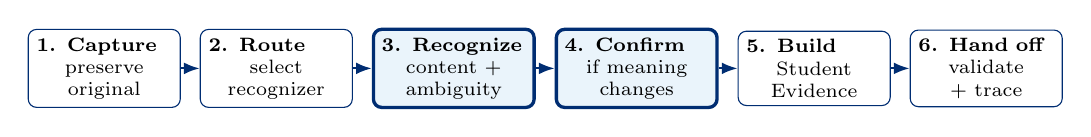
\begin{tikzpicture}[
  node distance=.24cm,
  box/.style={draw=HopkinsBlue,rounded corners=3pt,fill=white,align=center,text width=1.72cm,minimum height=.92cm,inner sep=3pt,font=\scriptsize},
  focus/.style={draw=HopkinsBlue,very thick,rounded corners=3pt,fill=PaleBlue,align=center,text width=1.83cm,minimum height=.92cm,inner sep=3pt,font=\scriptsize},
  arrow/.style={-{Latex[length=2mm]},thick,draw=HopkinsBlue}]
\node[box] (capture) {\textbf{1. Capture}\newline preserve original};
\node[box,right=of capture] (route) {\textbf{2. Route}\newline select recognizer};
\node[focus,right=of route] (read) {\textbf{3. Recognize}\newline content + ambiguity};
\node[focus,right=of read] (confirm) {\textbf{4. Confirm}\newline if meaning changes};
\node[box,right=of confirm] (build) {\textbf{5. Build}\newline Student Evidence};
\node[box,right=of build] (handoff) {\textbf{6. Hand off}\newline validate + trace};
\draw[arrow] (capture)--(route);
\draw[arrow] (route)--(read);
\draw[arrow] (read)--(confirm);
\draw[arrow] (confirm)--(build);
\draw[arrow] (build)--(handoff);
\end{tikzpicture}
\vspace{.65em}
\begin{columns}[T,onlytextwidth]
\column{.31\textwidth}
\begin{block}{Submission}
The original student input and stable course, question, session, turn, and attempt links.
\end{block}
\column{.32\textwidth}
\begin{block}{Recognition}
The interpretation, alternatives, uncertainty, and corrections. For handwriting below 300 DPI or 2000 px on its long edge, create a derived 300-DPI/2$\times$ copy, then deskew, denoise, and enhance contrast/sharpness. Log every transform; never overwrite the original.
\end{block}
\column{.34\textwidth}
\begin{block}{Evidence}
Confirmed factual work and history, without correctness, mastery, or misconception labels.
\end{block}
\end{columns}
\specnote{student-interaction.md}{\S\S6--10, 12 and 16; \texttt{interfaces.md} \S\S4--7}
\end{frame}

% 1:20
\begin{frame}{Outputs: what leaves and where it goes}
\footnotesize
\begin{tabularx}{\textwidth}{@{}P{.25\textwidth}P{.29\textwidth}Y@{}}
\toprule
\textbf{Output} & \textbf{Receiving module} & \textbf{Contract} \\
\midrule
\texttt{StudentSubmission} & Recognizer, evidence builder, session state & Original input with a stable ID and input type. \\
\addlinespace
Recognition result/correction & Delivery confirmation UI; evidence builder & Raw interpretation stays separate from confirmed content. \\
\addlinespace
\texttt{StudentEvidence} & Learner State/Tutoring Engine & Validated observable facts and history; no diagnosis. \\
\addlinespace
Retrieval request & RAG/Course Retrieval & Minimum question/evidence context under the agreed routing contract. \\
\addlinespace
Trace event & Session state/diagnostics & Handoff status, record versions, timing, and optional cost. \\
\addlinespace
Confirmation or retry request & Delivery Layer/Avatar & Focused request for information needed to continue. \\
\bottomrule
\end{tabularx}
\vspace{.4em}
\centering
Every output identifies its producer, consumer, schema version, status, and source records.
\specnote{student-interaction.md}{\S6 and \S14; \texttt{interfaces.md} \S\S4--7, 9--13}
\end{frame}

% 2:00
\begin{frame}{Generic example: one tutoring turn}
\scriptsize
\centering
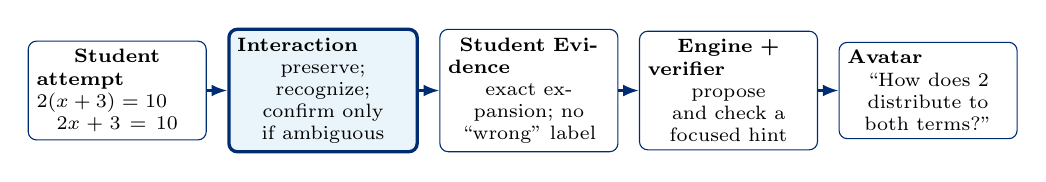
\begin{tikzpicture}[
  node distance=.26cm,
  box/.style={draw=HopkinsBlue,rounded corners=3pt,fill=white,align=center,text width=2.05cm,minimum height=.95cm,inner sep=3pt,font=\scriptsize},
  mine/.style={draw=HopkinsBlue,very thick,rounded corners=3pt,fill=PaleBlue,align=center,text width=2.18cm,minimum height=.95cm,inner sep=3pt,font=\scriptsize},
  arrow/.style={-{Latex[length=2mm]},thick,draw=HopkinsBlue}]
\node[box] (s1) {\textbf{Student attempt}\newline $2(x+3)=10$\newline $2x+3=10$};
\node[mine,right=of s1] (cap) {\textbf{Interaction}\newline preserve; recognize; confirm only if ambiguous};
\node[box,right=of cap] (ev) {\textbf{Student Evidence}\newline exact expansion; no ``wrong'' label};
\node[box,right=of ev] (eng) {\textbf{Engine + verifier}\newline propose and check a focused hint};
\node[box,right=of eng] (del) {\textbf{Avatar}\newline ``How does 2 distribute to both terms?''};
\draw[arrow] (s1)--(cap);
\draw[arrow] (cap)--(ev);
\draw[arrow] (ev)--(eng);
\draw[arrow] (eng)--(del);
\end{tikzpicture}
\vspace{.55em}
\begin{columns}[T,onlytextwidth]
\column{.48\textwidth}
\begin{block}{Context received before the attempt}
\begin{itemize}
\item Active course and question identifiers
\item Prompt: solve $2(x+3)=10$
\item Expected response mode
\item Display-safe concept and constraint references
\end{itemize}
\end{block}
\column{.49\textwidth}
\begin{block}{Next response}
The student revises to $2x+6=10$, then $x=2$. Interaction creates new evidence linked to the earlier attempt and the hint; neither attempt is overwritten.
\end{block}
\end{columns}
\vspace{.3em}
\centering
\textbf{Visible progress:} one trace connects context, original work, assistance, delivery, and revision across module boundaries.
\specnote{student-interaction.md}{\S\S8, 14, 16--17; \texttt{architecture.md} \S5}
\end{frame}

% 1:20
\begin{frame}{Ambiguity and failure behavior}
\scriptsize
\begin{tabularx}{\textwidth}{@{}P{.27\textwidth}P{.20\textwidth}Y@{}}
\toprule
\textbf{Condition} & \textbf{Status} & \textbf{Required response} \\
\midrule
$x_2$ versus $x^2$, or another meaning-changing uncertainty & \texttt{unconfirmed} & Show the relevant region and candidates; require student edit or confirmation. \\
\addlinespace
No usable content after enhancement, or unsupported input & \texttt{invalid}/\texttt{failed} & Preserve according to policy, request a clearer rescan or supported retry, and create no usable evidence. \\
\addlinespace
Only part of the work is recognized & \texttt{partial} & Mark missing regions; continue only if downstream policy accepts partial evidence. \\
\addlinespace
Course/question reference is absent & \texttt{context\_missing} & Preserve the submission but stop the tutoring handoff until repaired. \\
\addlinespace
Reasoning is rejected or cannot be checked & Verification blocked & Return to the Tutoring Engine or retry verification; do not deliver as approved. \\
\addlinespace
Delivery or another handoff fails & Recoverable failure & Retry or request an allowed alternative without changing the tutoring decision. \\
\bottomrule
\end{tabularx}
\vspace{.4em}
\centering
\alert{Recognition never silently repairs a student's mathematical mistake.}
\specnote{student-interaction.md}{\S\S10--11, 13--16; \texttt{README.md} \S7}
\end{frame}

% 1:25
\begin{frame}{Verify every student and model step}
\small
\centering
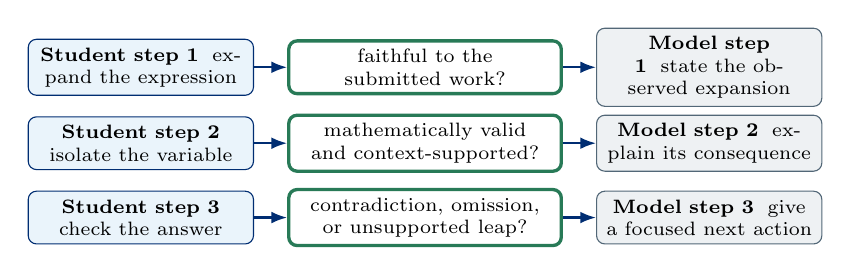
\begin{tikzpicture}[
  node distance=.26cm and .42cm,
  studentstep/.style={draw=HopkinsBlue,rounded corners=3pt,fill=PaleBlue,align=center,text width=2.65cm,minimum height=.67cm,inner sep=3pt,font=\scriptsize},
  check/.style={draw=Success,very thick,rounded corners=3pt,fill=white,align=center,text width=3.25cm,minimum height=.67cm,inner sep=3pt,font=\scriptsize},
  modelstep/.style={draw=Muted,rounded corners=3pt,fill=LightGray,align=center,text width=2.65cm,minimum height=.67cm,inner sep=3pt,font=\scriptsize},
  arrow/.style={-{Latex[length=2mm]},thick,draw=HopkinsBlue}]
\node[studentstep] (s1) {\textbf{Student step 1}\; expand the expression};
\node[studentstep,below=of s1] (s2) {\textbf{Student step 2}\; isolate the variable};
\node[studentstep,below=of s2] (s3) {\textbf{Student step 3}\; check the answer};
\node[check,right=of s1] (c1) {faithful to the submitted work?};
\node[check,right=of s2] (c2) {mathematically valid and context-supported?};
\node[check,right=of s3] (c3) {contradiction, omission, or unsupported leap?};
\node[modelstep,right=of c1] (m1) {\textbf{Model step 1}\; state the observed expansion};
\node[modelstep,right=of c2] (m2) {\textbf{Model step 2}\; explain its consequence};
\node[modelstep,right=of c3] (m3) {\textbf{Model step 3}\; give a focused next action};
\draw[arrow] (s1)--(c1); \draw[arrow] (c1)--(m1);
\draw[arrow] (s2)--(c2); \draw[arrow] (c2)--(m2);
\draw[arrow] (s3)--(c3); \draw[arrow] (c3)--(m3);
\end{tikzpicture}
\vspace{.45em}
\begin{columns}[T,onlytextwidth]
\column{.48\textwidth}
\begin{block}{Pass only when}
Every student step is represented accurately, every model step has support, and the response remains consistent with the question and course passages.
\end{block}
\column{.49\textwidth}
\begin{block}{Otherwise}
Return the failed step, reason, and supporting references to the Tutoring Engine for revision. Unchecked or failed output is not delivered as approved.
\end{block}
\end{columns}
\vspace{.3em}
\centering
\textbf{The verification layer checks reasoning; it does not choose pedagogy or rewrite student work.}
\end{frame}

% 1:00
\begin{frame}{Capture and evidence targets}
\footnotesize
\begin{tabularx}{\textwidth}{@{}P{.24\textwidth}Y P{.25\textwidth}@{}}
\toprule
\textbf{Area} & \textbf{Measure} & \textbf{Initial target} \\
\midrule
Text/math recognition & Normalized equation exact match; symbol error rate (SER) & Exact $\geq90\%$; SER $\leq5\%$ \\
Recorded voice & Word error rate on the confirmed transcript & WER $\leq10\%$ \\
Handwriting enhancement & Original retention; logged transforms; low-resolution exact-match gain; enhancement-induced symbol error & $100\%$ retained/logged; gain $\geq10$ percentage points; induced error $\leq1\%$ \\
Evidence integrity & Required ID/link validity; raw/corrected separation; overwritten originals & $100\%$ valid/separate; zero overwrites \\
Ambiguity handling & Recall and precision on meaning-changing ambiguity; confirmations per submission & Recall $\geq95\%$; precision $\geq80\%$; median $\leq1$ confirmation \\
\bottomrule
\end{tabularx}
\vspace{.2em}
\begin{block}{How to calculate recognition quality}
Exact match compares normalized expressions. SER $=$ symbol edit distance divided by reference-symbol count. Enhancement gain $=$ post-enhancement exact-match rate minus the unenhanced rate on the same low-resolution pages.
\end{block}
\specnote{student-interaction.md}{\S\S9--11 and 15--17}
\end{frame}

% 1:00
\begin{frame}{Reasoning and operation targets}
\footnotesize
\begin{tabularx}{\textwidth}{@{}P{.24\textwidth}Y P{.25\textwidth}@{}}
\toprule
\textbf{Area} & \textbf{Measure} & \textbf{Initial target} \\
\midrule
Student-work coverage & Recognized student steps represented in the verification trace & $100\%$ of steps accounted for \\
Model-step validity & Mathematically valid model steps divided by all proposed model steps & $\geq95\%$ \\
Grounding and safety & Supported-claim precision; false-accept rate; contradiction rate & Grounding $\geq95\%$; false accepts $\leq2\%$; contradictions $\leq1\%$ \\
Turn completion & Tutoring turns ending in a valid Delivery Result or structured recoverable status & $\geq95\%$ \\
Latency and accounting & End-to-end p95 latency; turns with latency and cost recorded & Typed $\leq8$s; handwriting $\leq25$s; accounting coverage $\geq99\%$ \\
\bottomrule
\end{tabularx}
\vspace{.2em}
\begin{block}{Tail-risk target}
Define turn loss on $[0,1]$ from math error, unsupported claims, unresolved ambiguity, and failed handoffs. Target $\mathrm{CVaR}_{95}\leq0.20$, where $\mathrm{CVaR}_{95}$ is mean loss in the worst 5\% of turns. Recalibrate after the first baseline.
\end{block}
\specnote{student-interaction.md}{\S\S15--17; \texttt{README.md} \S\S7, 10}
\end{frame}

% 1:00
\begin{frame}{This week's progress and next decisions}
\begin{columns}[T,onlytextwidth]
\column{.48\textwidth}
\begin{block}{Made concrete this week}
\begin{itemize}
\item V1 input boundary and ownership
\item Named producers and consumers
\item Submission, recognition, and evidence contracts
\item Ambiguity and failure behavior
\item Generic end-to-end tutoring trace
\item Proposed reasoning-verification gate
\end{itemize}
\end{block}
\column{.49\textwidth}
\begin{block}{Still open}
\begin{itemize}
\item Minimum evidence accepted by the engine
\item Timeout and retry behavior between modules
\end{itemize}
\vspace{.35em}
These are the only remaining interface decisions identified for this module.
\end{block}
\end{columns}
\vspace{.35em}
\centering
\textbf{Next milestone:} implement one typed tutoring loop, then add handwriting, stylus, and recorded voice through the same contracts.
\end{frame}

\end{document}
